\documentclass{article}

\usepackage{fullpage}
\usepackage{amsmath}
\usepackage{graphicx}
\usepackage[utf8]{inputenc}
\usepackage{pdfpages}
\usepackage{graphicx}
\usepackage{multicol}
\usepackage{tikz}
\usepackage{pgfplots}
\pgfplotsset{compat=1.12}


\title{Examen final de Cálculo Diferencial}
\author{M. en C. Reinaldo Arturo Zapata Peña}

\begin{document}
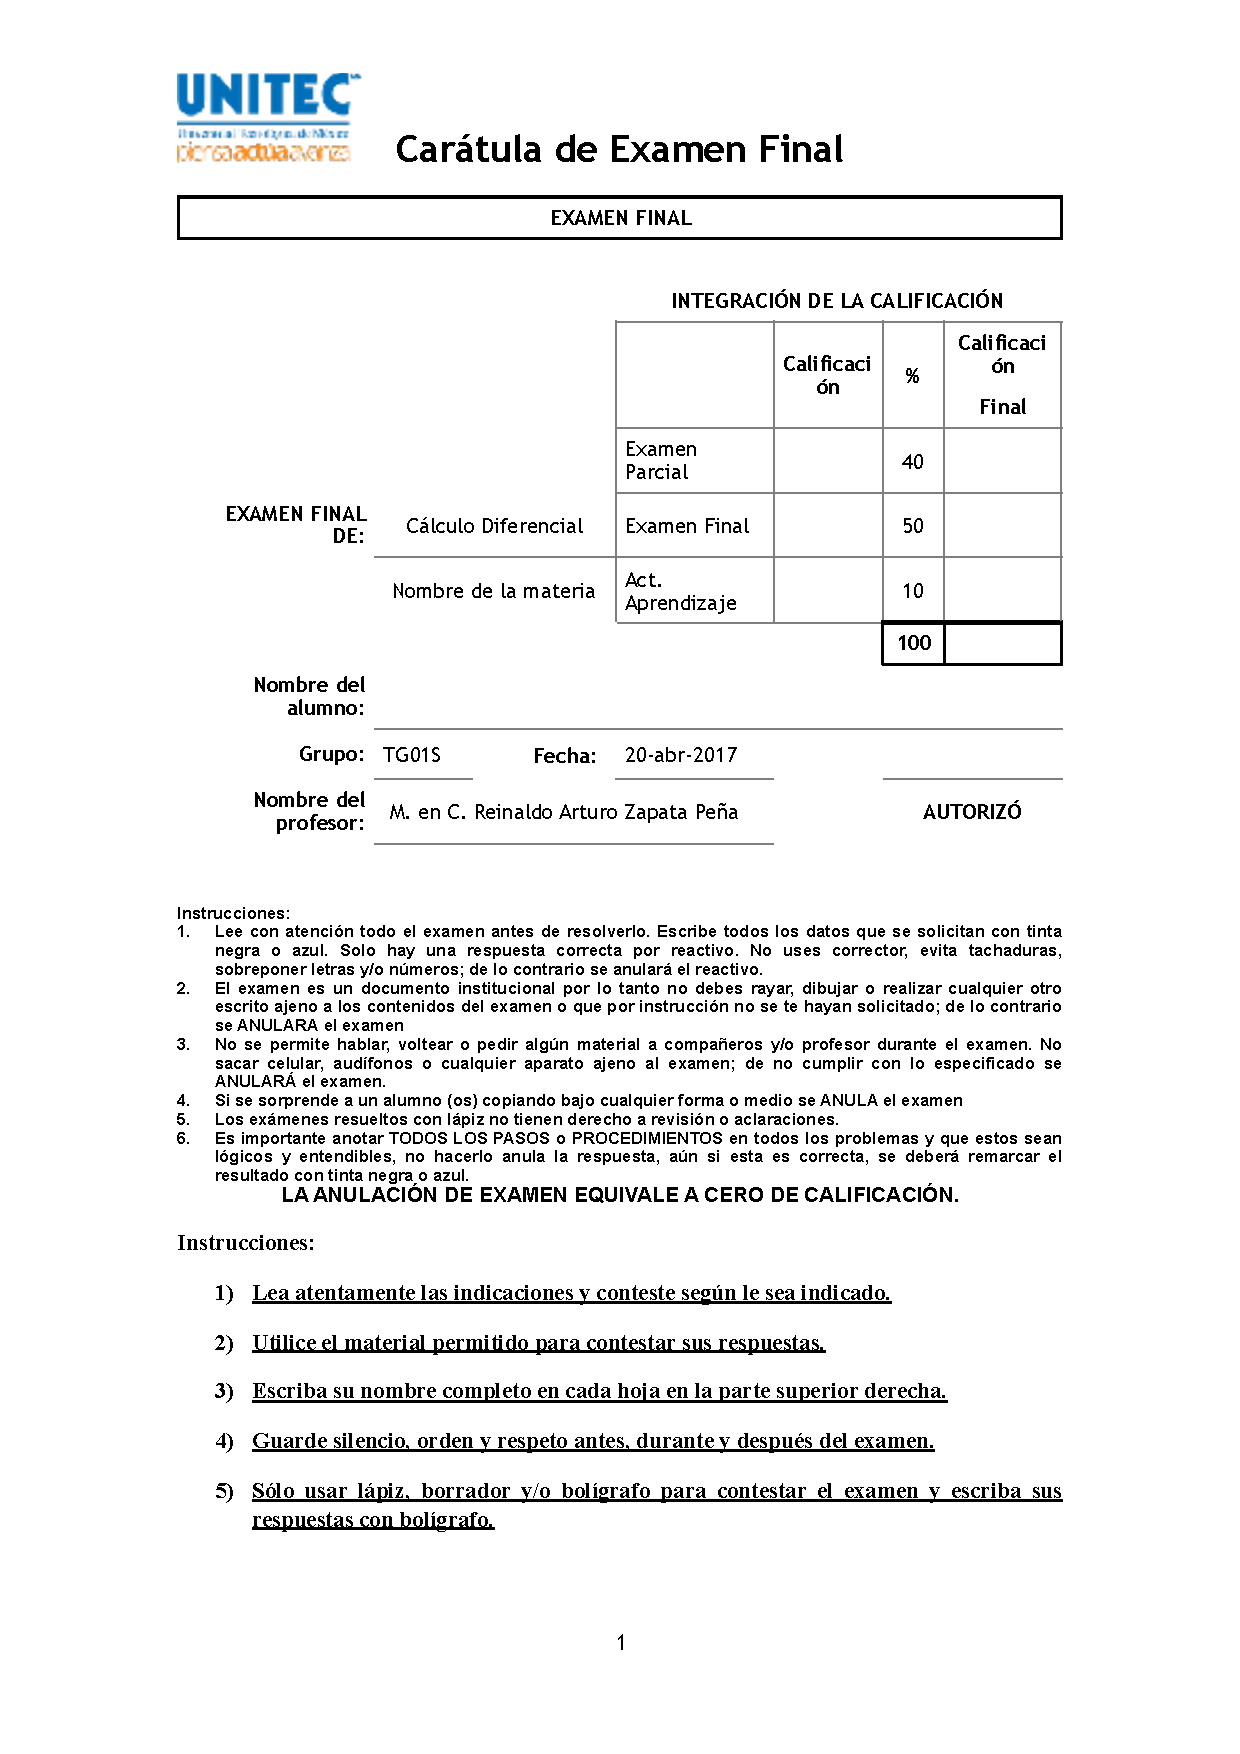
\includepdf[pages=-]{car-final-calc}

\section{Teoría} % (fold)
\label{sec:teoria}


\begin{figure}[b]
    \centering
  \begin{tikzpicture}
    \begin{axis}[
     x=60, y=30, clip=false, xmin=-0.30,xmax=2.2*pi, xlabel= $x$,
     ylabel=$f(x)$, ymin=-2.2,ymax=2.7, axis lines=middle,
     xtick={0,1.57,3.14,4.71,6.28}, xticklabel style = {fill=white},
     xticklabels={$0$, $\displaystyle\frac{\pi}{2}$,
     $\displaystyle\pi\,$,$\,\,\,\displaystyle\frac{3\pi}{2}$,$\,2\pi$}, set
     layers = axis on top ]
     \draw (axis cs:0,1) -- (axis cs:6.28,1);
     \draw (axis cs:0,2) -- (axis cs:6.28,2);
     \draw (axis cs:0,-1) -- (axis cs:6.28,-1);
     \draw (axis cs:0,-2) -- (axis cs:6.28,-2);
     \draw (axis cs:1.57,2) -- (axis cs:1.57,-2);
     \draw (axis cs:3.14,2) -- (axis cs:3.14,-2);
     \draw (axis cs:4.71,2) -- (axis cs:4.71,-2);
     \draw (axis cs:6.28,2) -- (axis cs:6.28,-2);
     \draw (axis cs:0.78,2) -- (axis cs:0.78,-2);
     \draw (axis cs:2.36,2) -- (axis cs:2.36,-2);
     \draw (axis cs:3.93,2) -- (axis cs:3.93,-2);
     \draw (axis cs:5.50,2) -- (axis cs:5.50,-2);
    \end{axis}
  \end{tikzpicture}
    \caption{especio  para graficar funciones.}
    \label{fig:graficar}
\end{figure}
\begin{enumerate}
\item Explique matemáticamente qué es una función par e impar.
\hfill \textbf{6 puntos.}

\item Haciendo uso de la figura \ref{fig:graficar}, haga un bosquejo de las
funciones $f(x)=\cos(2x)$ y $g(x)=2\sin(x)$ para el intervalo $0 \leq x \leq
2\pi$. Identifica cada una de ellas etiquet\'andolas.
\hfill \textbf{6 puntos.}

\item Explique con sus palabras que interpretación geométrica y matemática tiene
la derivada de una función.

\hfill \textbf{6 puntos.}

\item Si para una recta tangencial a una función $f(x)$ se conoce el punto
($a$,$f(a)$) y la pendiente de la recta tangente $m_{\text{tan}}$, escriba el
procedimiento para encontrar la recta perpendicular a la función en dicho punto.
\hfill \textbf{6 puntos.}

\item Explique con sus palabras que establece el teorema de l'H\^opital y las
situaciones en las que se puede utilizar.
\hfill \textbf{6 puntos.}

\end{enumerate}

% section teoría (end)



\section{Problemas} % (fold)
\label{sec:problemas}

\begin{enumerate}

\item Sea la función $f(x)= 2x^{2} -3x + 8$ encuentre las rectas tangente y
perpendicular a dicha función en el punto $x=4$. Determine para ambos casos si
la recta forma un ángulo mayor o menor a 90$^{\circ}$ respecto al eje de las $x$
midiendo en sentido contrario a las manecillas del reloj.
\hfill \textbf{9 puntos.}

\item Dadas las siguientes funciones, 
\hfill \textbf{9 puntos.}

\begin{align}
f(x) &= \frac{x^{2} - 4x  + 4 }{x-2}, \label{eq:lim1}
\\
g(x) &= \frac{\sin^{2}(x)}{x^{2}-25}, \label{eq:lim2}
\end{align}
encuentre los puntos para los cuales estas funciones son indeterminadas.

\item Utilizando las funciones del inciso anterior, determine si existe el
límite para la Ec. \eqref{eq:lim1} cuando $x \rightarrow 2$ y el límite para la
Ec. \eqref{eq:lim2} cuando $x \rightarrow 5$. 
\hfill \textbf{9 puntos.}

\item Utilizando la regla de l'H\^opital, determine el límite de las siguientes
funciones
\hfill \textbf{9 puntos.}
\begin{align}
\label{eq:lop1}\lim_{x \rightarrow 0} &\frac{\sin^{2}(x)}{x^{2}}  \\
\label{eq:lop2}\lim_{x \rightarrow \infty} &\frac{\ln(x)}{e^x} \\
\label{eq:lop3}\lim_{x \rightarrow 0} &\frac{1-e^{x}}{x}
\end{align}

\item Usando la regla de la cadena y las reglas de derivación encuentre la
derivada de las siguientes funciones.

\hfill \textbf{9 puntos.}

\noindent
\begin{minipage}{0.5\linewidth}
\begin{align}
\label{eq:f(x)} f(x) &= \tan(x)  \\
\label{eq:g(x)} g(x) &= \ln(x^{2})e^{2x^{3}}  \\
\label{eq:h(x)} h(x) &= \frac{\sin(2x)}{e^x}  
\end{align}
\end{minipage}%
\begin{minipage}{0.5\linewidth}
\begin{align}
\label{eq:i(x)} i(x) &= 3x^5\cos(2x) \\
\label{eq:j(x)} j(x) &= \sin^{3}(2x^{2})  \\
\label{eq:k(x)} k(x) &= \frac{1}{e^{2x^{5}}}  
\end{align}
\end{minipage}

\item Si la posición de un sistema en movimiento está dada por la función
\hfill \textbf{8 puntos.}
\begin{equation}\label{eq:poscion}
x(t)= 5t^{2} - 6t + 8
\end{equation}
determine la velocidad y la aceleración de la partícula en función del tiempo.

\item Encuentre la tercera derivada de la Ec. \eqref{eq:k(x)}.
\hfill \textbf{9 puntos.}


\end{enumerate}
% section problemas (end)

%%%%%%%%%%%%%%%%%%%%%%%%%%%%%%%%%%%%%%%%%%%%%%%%%%%%%%%%%%%%%%%%%%%%%%%%%%%%%%%%
%%%%%%%%%%%%%%%%%%%%%%%%%%%%%%%%%%%%%%%%%%%%%%%%%%%%%%%%%%%%%%%%%%%%%%%%%%%%%%%%

\clearpage
\setcounter{section}{0}

\begin{center}
{\sc \huge Respuestas}
\end{center}


\section{Teoria} % (fold)
\label{sec:resteoria}

\begin{enumerate}

\item Funci\'on par: $f(-x) = f(x) $. Función impar: $f(-x)=-f(x)$.

\item Gr\'afica: $f(x)=\cos(2x)$; $g(x)=2\sin(x)$.
\begin{figure}[h!]
    \centering
  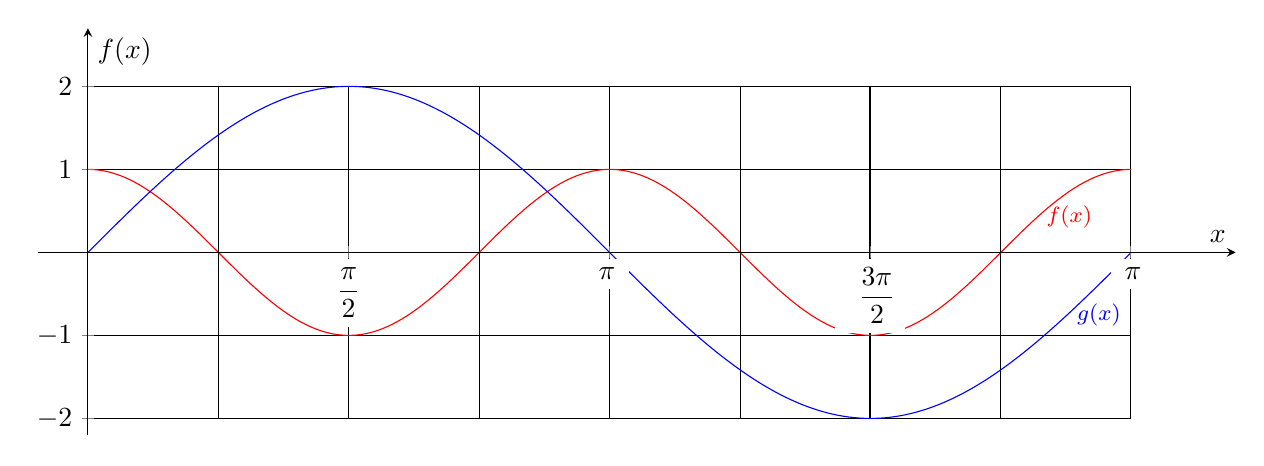
\begin{tikzpicture}
    \begin{axis}[
     x=60,
     y=30,
     clip=false,
     xmin=-0.30,xmax=2.2*pi,
     xlabel= $x$,
     ylabel=$f(x)$,
     ymin=-2.2,ymax=2.7,
     axis lines=middle,
     xtick={0,1.57,3.14,4.71,6.28},
     xticklabel style = {fill=white},
     xticklabels={$0$, $\displaystyle\frac{\pi}{2}$, $\displaystyle\pi\,$,$\,\,\,\displaystyle\frac{3\pi}{2}$,$\,\pi$},
     set layers = axis on top
     ]
     \draw (axis cs:0,1) -- (axis cs:6.28,1);
     \draw (axis cs:0,2) -- (axis cs:6.28,2);
     \draw (axis cs:0,-1) -- (axis cs:6.28,-1);
     \draw (axis cs:0,-2) -- (axis cs:6.28,-2);
     \draw (axis cs:1.57,2) -- (axis cs:1.57,-2);
     \draw (axis cs:3.14,2) -- (axis cs:3.14,-2);
     \draw (axis cs:4.71,2) -- (axis cs:4.71,-2);
     \draw (axis cs:6.28,2) -- (axis cs:6.28,-2);
     \draw (axis cs:0.785,2) -- (axis cs:0.785,-2);
     \draw (axis cs:2.36,2) -- (axis cs:2.36,-2);
     \draw (axis cs:3.93,2) -- (axis cs:3.93,-2);
     \draw (axis cs:5.497,2) -- (axis cs:5.497,-2);
    \addplot[domain=0:2*pi,samples=200,red]{cos(deg(2*x))}
                                node[right,pos=0.92,font=\footnotesize]{$f(x)$};
    \addplot[domain=0:2*pi,samples=200,blue]{2*sin(deg(x))}
                                node[right,pos=0.92,font=\footnotesize]{$g(x)$};
    \end{axis}
  \end{tikzpicture}
    % \caption{especio  para graficar funciones.}
    \label{fig:graficar2}
\end{figure}

\item La derivada de una función evaluada en un punto $a$ da como resultado la 
pendiente de la recta tangente a la curva de la función en ese mismo punto. La 
derivada de una función respecto a una de sus variables puede ser interpretada 
como la razón de cambio de la función respecto a dicha variable.

\item La recta perpendicular está dada por la ecuación 
\begin{align*}
m_{\perp} &= - \frac{1}{m_{\tan}} \\
y - f(a) &= m_{\perp} (x - a)
\end{align*}

\item La regla o teorema de l'H\^opital establece que el límite del cociente de
dos funciones $f(x)$ y $g(x)$ cuando $x$ tiende a un valor dado $a$, se puede 
obtener mediante 
\begin{align*}
\lim_{x \rightarrow a} \frac{f(x)}{g(x)}= 
\lim_{x \rightarrow a}\frac{f'(x)}{g'(x)}     
\end{align*} 
siempre y cuando se cumpla uno de los siguientes criterios
\begin{align*}
\lim_{x \rightarrow a} \frac{f(x)}{g(x)}= \frac{\infty}{\infty} \\
\lim_{x \rightarrow a} \frac{f(x)}{g(x)}= \frac{0}{0}
\end{align*} 

\end{enumerate}
% section resteoria (end)

\section{Problemas} % (fold)
\label{sec:resproblemas}
\begin{enumerate}

\item Ecuación de la recta tangente:
\begin{align*}
P(x,y) &= (4,f(4)) = (4,28) \\
m_{\tan} &= f'(4) = 13 \\
y - 28 &= 13(x-4) \\
y &= 13x -28
\end{align*}
Ecuación de la recta perpendicular:
\begin{align*}
P(x,y) &= (4,f(4)) = (4,28) \\
m_{\perp} &=- \frac{1}{f'(4)} =-\frac{1}{13} \\
y - 28 &= -\frac{1}{13}(x-4) \\
y &= - \frac{x}{13} + \frac{368}{13}
\end{align*}

\item Puntos de indeterminación: 

Para la Eq. \eqref{eq:lim1}: $x=-5$ \\
Para la Eq. \eqref{eq:lim2}: $x = \pm 5$

\item Límites: 

Para la Eq. \eqref{eq:lim1}: $\lim_{x \rightarrow 2}f(x) = 0$ \\
Para la Eq. \eqref{eq:lim2}: No existe el límite.

\item Regla de l'H\^opital:

Para la Eq. \eqref{eq:lop1}: lím = $\frac{1}{2}$  \\
Para la Eq. \eqref{eq:lop2}: lím = 0  \\
Para la Eq. \eqref{eq:lop3}: lím = -1 

\item Derivadas:
\begin{align*}
f'(x) &= \frac{1}{\cos^2(x)} = \csc^{2}(x) \\
g'(x) &= \ln(x^{2})e{2x^{3}}(6x) + \frac{e^{2x^{3}}}{x^2}(2x) \\
      &= 6x \ln(x^{2})e^{2x^{3}} + \frac{2e^{2x^3}}{x^2} \\
h'(x) &= - \sin(2x)e^{-x} + 2e^{-x} \cos{(2x)} \\
i'(x) &= 15x^{4} \cos(2x) -6x^{5}sin(2x) \\
j'(x) &= 12x \sin^{2}(2x^{2}) \cos(2x^{2}) \\
k'(x) &= -10x^{4}e^{-2x^{5}}
\end{align*}

\item Velocidad y aceleración:
\begin{align*}
v(t) &= \frac{dx}{dt} = 10t -6 \\
a(t) &= \frac{d^2x}{dt^2} = 10
\end{align*}

\item Tercera derivada
\begin{align*}
k''(x)  &= 100x^{4} e^{2x^{5}} -40x^3 e^{2x^{5}} \\
k'''(x) &= -1000x^{4} e^{2x^{5}} + 400 x^{7} e^{2x^{5}} + 
            400x^{3} e^{2x^{5}} - 120 x^{2} e^{2x^{5}} \\
        &= (-1000x^{4} + 400 x^{7} + 400x^{3} - 120 x^{2}) e^{2x^{5}} \\
\end{align*}

\end{enumerate}
% section resproblemas (end)

\end{document}

(3^2 -4*3 +4)/(3+5)

